\subsection*{Review Exercise 1.314}

\subsubsection*{Instruction}

State the domain and range of the function $ h(x) = \frac{1}{x + 4} $.

\subsubsection*{Solution}

We can start by sketching a graph of the function $h(x)$ to improve our understanding of its characteristics.

\begin{figure}[H]
  \centering
  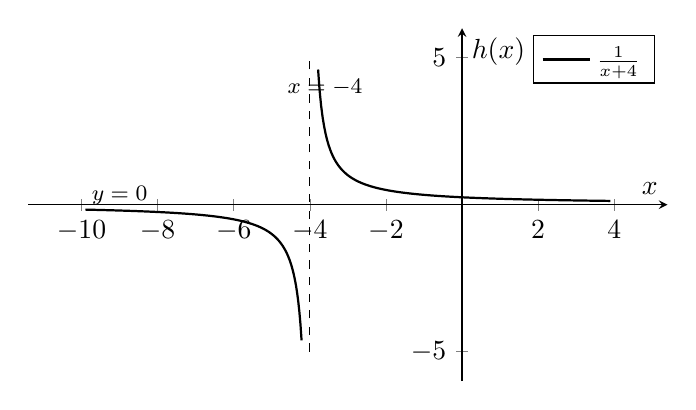
\begin{tikzpicture}
    \begin{axis}[
        axis lines=middle,
        xlabel=\( x \),
        ylabel=\( h(x) \),
        xmin=-10, xmax=4,  % extended x-axis to show more
        ymin=-5, ymax=5,
        samples=200,
        domain=-9.9:3.9,
        restrict y to domain=-5:5,
        legend style={
          draw=black,
          fill=white,
          font=\small,
          at={(0.98,0.98)},
          anchor=north east
        },
        width=0.8\textwidth,
        height=0.5\textwidth,
        enlargelimits=true,
        clip=false,
      ]

      % Function plot
      \addplot[black, thick, domain=-9.9:-4.1] {1/(x + 4)};
      \addplot[black, thick, domain=-3.9:3.9] {1/(x + 4)};
      \addlegendentry{\( \frac{1}{x + 4} \)}

      % Vertical asymptote x = -4
      \draw[dashed] (axis cs:-4,-5) -- (axis cs:-4,5);
      \node at (axis cs:-3.6,4) {\footnotesize \( x = -4 \)};

      % Horizontal asymptote y = 0
      \draw[dashed] (axis cs:-10,0) -- (axis cs:4,0);
      \node at (axis cs:-9,0.3) {\footnotesize \( y = 0 \)};
    \end{axis}
  \end{tikzpicture}
  \caption{Graph of \( \frac{1}{x + 4} \). The function has a vertical asymptote at \( x = -4 \) and a horizontal asymptote at \( y = 0 \).}
  \label{fig:graph-h-of-x}
\end{figure}

To find the domain of $h$ we note that $ \frac{1}{x + 4} $ is defined when the denominator is nonzero, the domain is $\{x \mid x \ne -4\}$.

To find the range of $h$, we need to find the values of $y$ such that there exists a real number $x$ in the domain with the property that
\[\phantom{.} \frac{1}{x + 4} = y \text{.}\]

Solving this equation for $x$, we find that
\[ \phantom{.} x = \frac{1}{y} -4 \text{.} \]

Therefore, as long as $ y \ne 0 $, there exists a real number $ x $ in the domain such that $h(x) = y$. Thus the range is $\{y \mid y \ne 0\}$
\subsubsection*{Answer}

Domain: $\{x \mid x \ne -4\}$, range: $\{y \mid y \ne 0\}$.
